%% Begin slides template file
\documentclass[11pt,t,usepdftitle=false,aspectratio=169]{beamer}
%% ------------------------------------------------------------------
%% - aspectratio=43: Set paper aspect ratio to 4:3.
%% - aspectratio=169: Set paper aspect ratio to 16:9.
%% ------------------------------------------------------------------

\usetheme[nototalframenumber,foot,logo]{uibk}
%% ------------------------------------------------------------------
%% - foot: Add a footer line for conference name and date.
%% - logo: Add the university logo in the footer (only if 'foot' set).
%% - bigfoot/sasquatch: Larger font size in footer.
%% - nototalslidenumber: Hide the total number of slides (only if 'foot' set)
%% - license: Add CC-BY license symbol to title slide (e.g., for conference uploads)
%%   (TODO: At the moment no other licenses are supported.)
%% - licenseall: Add CC-BY license symbol to all subsequent slides slides
%% - url: use \url{} rather than \href{} on the title page
%% - nosectiontitlepage: switches off the behaviour of inserting the
%%   titlepage every time a \section is called. This makes it possible to
%%   use more than one section + thanks page and a ToC off by default.
%%   If the 'nosectiontitlepage' is set you can create UIBK title slides
%%   using the command '\uibktitlepage{}' in your document to create
%%   one or multiple title slides.
%% ------------------------------------------------------------------

%% ------------------------------------------------------------------
%% The official corporate colors of the university are predefined and
%% can be used for e.g., highlighting something. Simply use
%% \color{uibkorange} or \begin{color}{uibkorange} ... \end{color}
%% Defined colors are:
%% - uibkblue, uibkbluel, uibkorange, uibkorangel, uibkgray, uibkgraym, uibkgrayl
%% The frametitle color can be easily adjusted e.g., to black with
%% \setbeamercolor{titlelike}{fg=black}
%% ------------------------------------------------------------------

%\setbeamercolor{verbcolor}{fg=uibkorange}
%% ------------------------------------------------------------------
%% Setting a highlight color for verbatim output such as from
%% the commands \pkg, \email, \file, \dataset
%% ------------------------------------------------------------------


%% information for the title page ('short title' is the pdf-title that is shown in viewer's titlebar)
\title[Segfault Slayer]{Initial Presentation: Segfault Slayer}
\subtitle{Name is work in progress}
% \URL{www.uibk.ac.at/statistics}

\author[Schmölz Lukas, Schöpf Emanuel, Schweigl Dominik]{Schmölz Lukas, Schöpf Emanuel, Schweigl Dominik}
%('short author' is the pdf-metadata Author)
%% If multiple authors are required and the font size is too large you
%% can overrule the font size of author and url by calling:
%\setbeamerfont{author}{size*={10pt}{10pt},series=\mdseries}
%\setbeamerfont{url}{size*={10pt}{10pt},series=\mdseries}
%\URL{}
%\subtitle{}

% \footertext{{\LaTeX} beamer theme}
% \date{2017-07-25}

\headerimage{3}
%% ------------------------------------------------------------------
%% The theme offers four different header images based on the
%% corporate design of the university of innsbruck. Currently
%% 1, 2, 3 and 4 is allowed as input to \headerimage{...}. Default
%% or fallback is '1'.
%% ------------------------------------------------------------------

\begin{document}

%% ALTERNATIVE TITLEPAGE
%% The next block is how you add a titlepage with the 'nosectiontitlepage' option, which switches off
%% the default behavior of creating a titlepage every time a \section{} is defined.
%% Then you can use \section{} as it's originally intended, including a table of contents.
% \usebackgroundtemplate{\includegraphics[width=\paperwidth,height=\paperheight]{titlebackground.pdf}}
% \begin{frame}[plain]
%     \titlepage
% \end{frame}
% \addtocounter{framenumber}{-1}
% \usebackgroundtemplate{}

%% Table of Contents, if wanted:
%% this requires the 'nosectiontitlepage' option and setting \section{}'s as you want them to appear here.
%% Subsections and subordinates are suppressed in the .sty at the moment, search
%% for \setbeamertemplate{subsection} and replace the empty {} with whatever you want.
%% Although it's probably too much for a presentation, maybe for a lecture.
%% Please note: \maketitle allows you to render a uibk-style title page wherever needed
%% in the document even if 'nosectiontitlepage' option is set (note: \maketitle will not
%% create a new section and is therefore not included in \tableofcontents (if used).
% \maketitle
% \begin{frame}
%     \vspace*{1cm plus 1fil}
%     \tableofcontents
%     \vspace*{0cm plus 1fil}
% \end{frame}


%% this sets the first PDF bookmark and triggers generation of the title page
\section{Bookmark Title}

%% this just generates PDF bookmarks
\subsection{Overview}

% \section{Overview}

\begin{frame}
	\frametitle{Game Theme}

	\textbf{Game Idea:}
	\begin{itemize}
		\item Metroidvania-style 2D side-scroller
		\item Player fights programming concepts and bugs (mainly C++ related)
		\item Playful, Pixel-theme (e.g. ASCII-Art for textures)
	\end{itemize}

	\bigskip

	\textbf{Brainstorming Examples:}
	\begin{itemize}
		\item Infinite loop for Boss
		\item Segmentation faults for ability
		\item C++ xvalues as enemies
	\end{itemize}

\end{frame}

\begin{frame}
	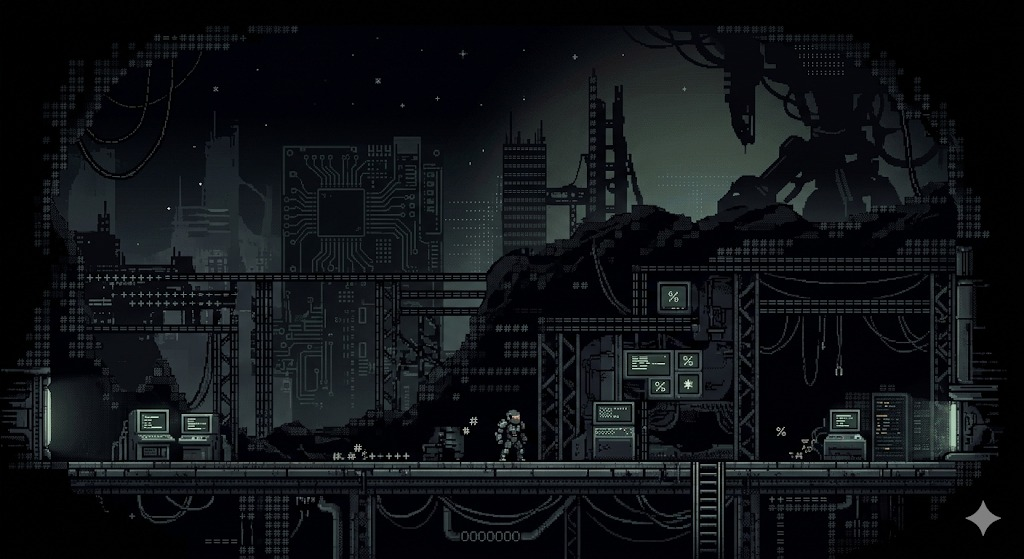
\includegraphics[width=\textwidth]{_images/concept_art.jpeg}
\end{frame}

\begin{frame}
	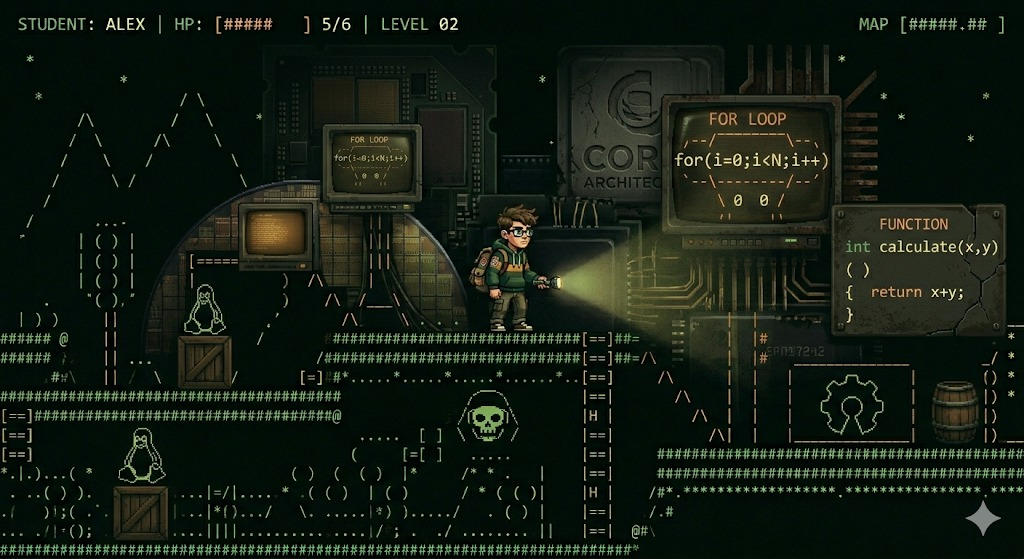
\includegraphics[width=\textwidth]{_images/concept_art_3.jpeg}
\end{frame}

\begin{frame}{Game Sprites}

	\begin{columns}[T]

		% LEFT COLUMN: text
		\begin{column}{0.4\textwidth}
			\small
			\textbf{Sprite Creation with Pixellab}

			\vspace{1em}

			We use \textbf{Pixellab}, a generative AI tool for creating game sprites.

			\vspace{1em}

			It includes builders for:
			\begin{itemize}
				\item Characters
				\item Maps
				\item Animations
			\end{itemize}

		\end{column}

		% RIGHT COLUMN: images, right-aligned
		\begin{column}{0.5\textwidth}
			\begin{flushright}
				\vspace{-2em}

				
\includegraphics[width=0.45\linewidth]{_images/pixellab_dragon.png}

				\vspace{0.5em}

				
\includegraphics[width=0.45\linewidth]{_images/pixellab_golem.png}
			\end{flushright}
		\end{column}

	\end{columns}

\end{frame}


\subsection{Project Structure}

\begin{frame}
	\frametitle{Project Structure}

	\textbf{Directory Layout:}

	\begin{itemize}
		\item \file{assets/}
		\item \file{build/}
		\item \file{data/}
		\item \file{docs/}
		\item \file{saves/}
		\item \file{src/}
		      \begin{itemize}
			      \item \file{core/}
			      \item \file{entities/}
			      \item \file{rendering/}
			      \item \file{utils/}
			      \item \file{world/}
		      \end{itemize}
		\item \file{tests/}
	\end{itemize}

\end{frame}

\begin{frame}
	\frametitle{Development Setup}

	\textbf{Dev.-Stack:}
	\begin{itemize}
		\item Must: git, cmake, clang-format, vcpkg
		\item CI
		\item 1 Windows \& 2 Linux
		\item Assets: AI \& manual polishing
	\end{itemize}


	\textbf{Project Management:}
	\begin{itemize}
		\item Issues
		\item Milestones
		\item Weekly Meetings
	\end{itemize}

\end{frame}

\begin{frame}
	\frametitle{Dependencies}

	\textbf{Dependencies:}
	\begin{itemize}
		\item SFML
		\item tilson
		\item spdlog / plog
		\item Catch2
		\item imgui (maybe)
		\item glaze (maybe)
	\end{itemize}

\end{frame}

\begin{frame}
	\frametitle{Team Responsibilities}

	\textbf{Task Distribution:}
	\begin{itemize}
		\item (2) enemies - Lukas
		\item (1) menus - Lukas
		\item (2) two consecutive areas - Emanuel
		\item (1) save / load with dedicated save points (rooms) - Emanuel
		\item (1) map - Emanuel
		\item (2) basic movement - Dominik
		\item (1) one or more advanced movement mechanics - Dominik
		\item (1) main combat - Dominik
	\end{itemize}

\end{frame}

\end{document}

